\chapter{Spezielle Ansätze im Softwareengineering – Teil 1}
%\label{sec:Kap-4}

In diesem Kapitel und ähnlichen Kapiteln in späteren Kurseinheiten stellen wir besondere Ansätze aus dem Bereich des Softwareengineering kompakt auf wenigen Seiten vor. Diese zeichnen sich dadurch aus, dass sie entweder ein wenig außerhalb des Softwareengineering-Mainstreams ihrer Zeit standen oder stehen, teilweise als neuester Softwareengineering-Trend vermarktet wurden oder werden, heute (noch) keinen sehr großen Verbreitungsgrad besitzen oder ein sehr begrenztes Einsatzfeld haben, und sie einem trotzdem als Schlagworte – oft aber auch nicht mehr – des Öfteren begegnen, wenn man sich mit Softwareengineering beschäftigt. Sie sind alle irgendwo in dem großen Bereich zwischen Methode und Vorgehensmodell anzusiedeln – dementsprechend haben wir den sehr vagen Begriff \textbf{Ansatz} als Überschrift für dieses Kapitel gewählt. Eine Zuordnung der Ansätze zu den Kurseinheiten erfolgt anhand der Themenschwerpunkte der jeweiligen Kurseinheit, war aber nicht immer eindeutig zu treffen, weil manche Themen genauso gut auch in andere Kurseinheiten gepasst hätten. Die Hinweise zur (weiterführenden) Literatur zum entsprechenden Thema finden Sie jeweils am Ende des Abschnitts.

%--- Kapitel 4.1
\section{Realwelt-Objekte modellieren}
\label{sec:Kap-4.1}

Im objektorientierten Softwareengineering versucht man das (zukünftige) Softwareprodukt so zu gestalten, dass es sich an den Objekten und Strukturen der Domäne orientiert. Die UML bietet mit dem sogenannten \textit{Objektdiagramm}
\marginline{Objekt\-diagramm} 
die Möglichkeit, (Abstraktionen der) Objekte der Realwelt, ihre Eigenschaften und ihre Beziehungen zueinander in einer von UML vorgegebenen Syntax zu modellieren. Objektdiagramme können unterschiedlich umfangreich sein, auch eine Menge von Objekten ohne Verbindungen zueinander (wie in Abbildung~\ref{fig:objektdiagramm_unverbundene_objekte}) und selbst ein einziges aufgezeichnetes Objekt (wie in Abbildung~\ref{fig:objekt_in_uml-darstellung}) stellen Objektdiagramme dar. In der praktischen Anwendung im Softwareengineering beinhalten Objektdiagramme in der Regel aber mehrere verbundene Objekte. 

Zu modellierende Realwelt-Objekte \marginline{Objekt}
können Dinge sein, die man sehen oder anfassen kann, wie zum Beispiel eine Katze, ein Tisch, eine Person oder ein Stern, aber auch immaterielle Dinge, wie zum Beispiel ein Konto, eine Reise oder eine Vorlesung. In der UML-Notation werden Objekte als rechteckige Kästen dargestellt, die (mindestens, s.u.) einen Objektnamen enthalten.

\vspace{2mm} %%% für Druck

\begin{figure}[h!]
	\centering
	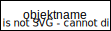
\includegraphics{Bilder/Kapitel-4/objekt_in_uml-darstellung.pdf}
	\caption{Ein Objekt in UML-Darstellung}
	\label{fig:objekt_in_uml-darstellung}
\end{figure}

Nach UML-Konvention wird der Objektname unterstrichen dargestellt. Üblich – obwohl die UML diesbezüglich keine Vorgaben macht – ist außerdem, dass Objektnamen mit einem Kleinbuchstaben beginnen und zentriert dargestellt werden. Innerhalb eines Diagramms müssen die Objektnamen eindeutig gewählt werden. Sollten innerhalb eines Diagramms trotzdem zwei Kästchen denselben Namen enthalten – die UML verbietet dies nicht –, so ist mit beiden Kästchen dasselbe Objekt gemeint. Die doppelte Darstellung eines Objekts wird vor allem in handschriftlich erstellten oder sehr umfangreichen Objektdiagrammen aus Lesbarkeitsgründen verwendet.

\vspace{2mm} %%% für Druck

\begin{figure}[h!]
	\centering
	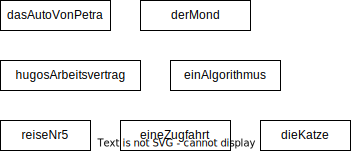
\includegraphics{Bilder/Kapitel-4/objektdiagramm_unverbundene_objekte.pdf}
	\caption{Ein Objektdiagramm mit sieben unverbundenen Objekten}
	\label{fig:objektdiagramm_unverbundene_objekte}
\end{figure}

Abbildung~\ref{fig:objektdiagramm_unverbundene_objekte} zeigt weitere Objekte in UML-Darstellung. Bei manchen wird aus dem Namen (relativ) deutlich, welches konkrete Realwelt-Objekt gemeint ist. So ist \linebreak \sttpUMLText{dasAutoVonPetra}, sofern man Petra kennt und sie nicht mehr als ein Auto besitzt, einem konkreten Realwelt-Auto zuordenbar. Für \sttpUMLText{reiseNr5} bedarf es dagegen schon der zusätzlichen Kenntnis des Kontexts (\zb die Auflistung von Reisen in einem Katalog), um eine Realwelt-Reise mit diesem Namen zu verbinden. Für Objekte wie \sttpUMLText{einAlgorithmus} oder \sttpUMLText{eineZugfahrt} und auch \sttpUMLText{dieKatze} lassen sich die gemeinten Realweltentsprechungen nicht bestimmen. 

Zumindest könnte man aber anhand der Namen der Objekte vielleicht auf die \textbf{Art} des Realwelt-Objekts schließen? So sollte es sich bei \sttpUMLText{dieKatze} doch wohl um eine Katze und nicht um einen Hund handeln? Doch vielleicht trägt mein Realwelt-Meerschweinchen – aus welchem Grund auch immer – den Namen \sttpUMLText{dieKatze} und meine Realwelt-Katze heißt stattdessen \sttpUMLText{pünktchen}. Der modellierten Abstraktion des Realwelt-Objekts kann man den Typ des Objekts in der bisher gewählten Darstellungsform also nicht ansehen. 

Um den Typ eines modellierten Realwelt-Objekts anzugeben, wird in der UML-Dar\-stel\-lung des Objekts der Objektname um die Angabe des Namens der \textit{Klasse}
\marginline{Klasse}
ergänzt (Abb.~\ref{fig:darstellung_objekt} rechts). Die Objektdarstellung ohne zusätzlichen Klassennamen (wie in Abb.~\ref{fig:darstellung_objekt} links und den vorherigen Abbildungen) ist nach UML-Regeln zulässig, sollte aus semantischen Gründen aber nur dann verwendet werden, wenn der Zielgruppe des Modells der Typ des Objekts bekannt ist.

\begin{figure}[h!]
	\centering
	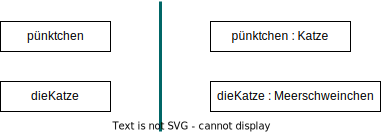
\includegraphics{Bilder/Kapitel-4/darstellung_objekt.pdf}
	\caption[Ein Katzen-Objekt namens \sttpUMLText{pünktchen} und ein Meerschweinchen-Objekt namens \sttpUMLText{dieKatze}]{Ein Objekt namens \sttpUMLText{pünktchen} und ein Objekt namens \sttpUMLText{dieKatze} (links). Ein Katzen-Objekt namens \sttpUMLText{pünktchen} und ein Meerschweinchen-Objekt namens \sttpUMLText{dieKatze} (rechts). Der senkrechte Strich in der Abbildung trennt die linke und die rechte Seite dieser Abbildung. Er ist nicht Bestandteil eines UML-Objektdiagramms.}
	\label{fig:darstellung_objekt}
\end{figure}


\sttpHinweiskasten{1.0}{CamelCase-Schreibweise}{Bezeichner (Namen) in Programmcode dürfen häufig keine Leerzeichen enthalten. Die sogenannte CamelCase-Schreibweise, bei der das erste Wort kleingeschrieben wird und alle folgenden jeweils mit einem Großbuchstaben beginnen, ist eine Möglichkeit, auch ohne Trennzeichen ausdrucksstärkere Bezeichner als \zb \sttpUMLText{auto1} und \sttpUMLText{auto2} zu verwenden. Die CamelCase-Schreibweise findet man auch in Domänenmodellen häufig, obwohl Domänenmodelle eigentlich noch von Implementierungsaspekten abstrahieren sollten und hier die Verwendung von Leerzeichen Realwelt-näher wäre. Die UML selber macht keine Vorgaben oder Einschränkungen bezüglich der Schreibweise der Namen, spezifische UML-Werkzeuge tun dies allerdings teilweise schon.}

Abbildung~\ref{fig:sechs_mal_katze} zeigt weitere Katzen-Objekte. Wichtig ist, dass jeweils ausschließlich die Angabe \sttpUMLText{:Katze} bestimmt, dass es sich um ein Objekt vom Typ Katze handelt. Die beiden unteren Objekte in der Abbildung sind sogenannte \textit{anonyme Objekte}.
\marginline{anonymes Objekt}
Diese Form der Darstellung wird verwendet, wenn man nicht ein konkretes, mit einem Namen versehenes, Katzen-Objekt modellieren möchte, sondern \textbf{irgendein} Objekt vom Typ Katze. Beachten Sie, dass auch ein anonymes Objekt nur genau \textbf{ein} Objekt ist. Es steht nicht stellvertretend für beliebig viele Katzen-Objekte. Im Unterschied zu benannten Objekten handelt es sich bei mehreren anonymen Objekten derselben Klasse im selben Objektdiagramm nach UML-Definition um \textbf{unterschiedliche} Objekte. Die beiden anonymen Katzen-Objekte in Abbildung~\ref{fig:sechs_mal_katze} modellieren daher zwei unterschiedliche Realwelt-Katzen, bei denen es aber für den Modellierungszweck irrelevant ist, um welche konkreten Realwelt-Katzen es sich handelt. Das Objekt mit Namen \sttpUMLText{eineKatze} ist dagegen kein anonymes Objekt, sondern modelliert genau diejenige Realwelt-Katze, die den Namen \sttpUMLText{eineKatze} trägt.

\begin{figure}[h!]
	\centering
	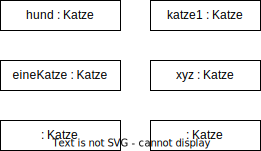
\includegraphics{Bilder/Kapitel-4/sechs_mal_katze.pdf}
	\caption{Vier benannte und zwei anonyme Objekte der Klasse \sttpUMLText{Katze}}
	\label{fig:sechs_mal_katze}
\end{figure}

Das Konzept der Klasse ist ein zentraler Bestandteil der objektorientierten Softwareentwicklung – auch wenn es einige wenige objektorientierte Programmiersprachen gibt (\zb JavaScript), die keine Klassen, sondern ausschließlich Objekte kennen. Sie kennen aus der objektorientierten Programmierung sicher die Definition einer Klasse als Bauplan bzw. Schablone für gleichartige Software-Objekte. Dabei wird die Klasse aus dem Blickwinkel der Programmcodeerstellung betrachtet. Aber was ist eigentlich eine Klasse, wenn wir mit dem Fokus der Realweltmodellierung hinsehen?

Abbildung~\ref{fig:klassenbegriff} greift das Beispiel mit Herrn Müller aus Abschnitt 3.2.1 (S.~\pageref{fig:mueller_lehrer_fussballer}) wieder auf. Aus dem Realwelt-Objekt Herr Müller wird durch entsprechende (unter\-schied\-liche) Abstraktion das modellierte Realwelt-Objekt Lehrer Müller oder das modellierte Realwelt-Objekt Fußballer Müller. Eine Klasse
\marginline{eine Klasse\\ ist die Beschrei\-bung einer Abstrak\-tion}
beschreibt genau diese Abstraktion zwischen dem Realwelt-Objekt und der Modellierung des Realwelt-Objekts. Die Klasse Lehrer definiert, welche Merkmale des Realwelt-Objekts für die Modellierung als Lehrer Müller relevant sind. Die Klasse Fußballer beschreibt die\-jenigen Merkmale des Realwelt-Objekts, die für die Modellierung als Fußballer Müller relevant sind.

\begin{figure}[h!]
	\centering
	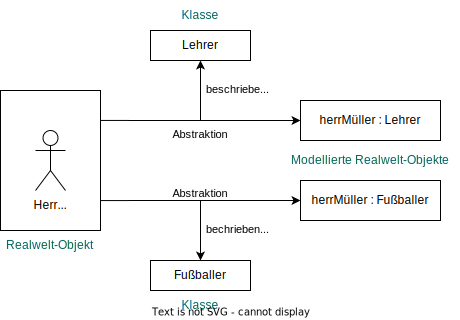
\includegraphics{Bilder/Kapitel-4/klassenbegriff_realweltmodellierung.pdf}
	\caption{Der Klassenbegriff aus Sicht der Realweltmodellierung}
	\label{fig:klassenbegriff}
\end{figure}


Zwei Aspekte zum Konzept der Klasse müssen wir an dieser Stelle noch ergänzen. Erstens gilt die in den Klassen Lehrer und Fußballer beschriebene Abstraktion natürlich nicht nur für das konkrete Realwelt-Objekt Herrn Müller, sondern für alle Realwelt-Objekte (Frau Schulze, Herr Özdemir, Frau Kinsombi,~\ldots), die modellierte Realwelt-Lehrer oder Realwelt-Fußballer werden sollen. Und zweitens beschreibt eine Klasse die Abstraktion zwischen Realwelt-Objekt und Modellierung eines solchen Realwelt-Objekts auch dann, wenn man (noch) gar kein modelliertes Objekt hat. So kann zum Beispiel eine Klasse Katze existieren, die definiert, wie man von einer Realwelt-Katze zu einer modellierten Realwelt-Katze kommen würde, ohne dass es ein modelliertes Katzen-Objekt gibt. Eine Klasse ist somit unabhängig von der Existenz der modellierten Objekte – umgekehrt gilt dies jedoch nicht.

\vspace{\baselineskip} %%% für Druck

\begin{figure}[h!]
	\centering
	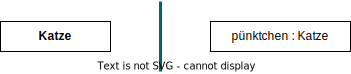
\includegraphics{Bilder/Kapitel-4/darstellung_klasse.pdf}
	\caption[Eine Klasse mit Namen \sttpUMLText{Katze} und ein Objekt dieser Klasse]{Eine Klasse mit Namen \sttpUMLText{Katze} (links) und ein Objekt dieser Klasse mit Namen \sttpUMLText{pünktchen} (rechts)}
	\label{fig:darstellung_klasse}
\end{figure}

\vspace{\baselineskip} %%% für Druck

Die UML-Darstellung einer Klasse ist sehr ähnlich zu der Darstellung eines Objekts. Es handelt sich ebenfalls um ein Rechteck, in dem (mindestens) der Klassenname eingetragen ist. Abbildung~\ref{fig:darstellung_klasse} zeigt links eine Klasse \sttpUMLText{Katze} und rechts ein modelliertes Katzen-Objekt namens \sttpUMLText{pünktchen}. Im Unterschied zu Objekten wird bei der Darstellung einer Klasse der Name nicht unterstrichen. Zudem ist es üblich, den Klassennamen mit einem Großbuchstaben zu beginnen und ihn zentriert und fett gedruckt zu setzen. Der Klassenname ist üblicherweise ein Substantiv im Singular und nicht im Plural. Wie auch bei den benannten Objekten gilt für Klassen in einem Diagramm, dass es sich bei der mehrfachen Darstellung einer Klasse per Defi\-ni\-tion um dieselbe Klasse handelt. Die mehrfache Darstellung von Klassen in einem Diagramm sollte man nur sehr dosiert anwenden, da die existierenden Beziehungen zwischen Klassen (s. Kap. \ref{sec:Kap-4.3}) mit jeder Dopplung einer Klasse im Diagramm weniger gut zu überblicken sind.

Wenn man Softwareprodukte, wie zum Beispiel die erwähnte Schulverwaltungssoftware entwickeln möchte, sind die konkreten Objekte der Realwelt wie Herr Müller meistens weniger interessant. Entscheidender ist, dass die Software später mit beliebigen Objekten eines bestimmten Typs (\zb Lehrer-Objekt) umgehen kann. Die Informationen zu den Merkmalen von Objekttypen finden sich in der objektorientierten Softwareentwicklung aber in den Klassen und nicht in den Objekten. Daher interessieren für die Softwareentwicklung vor allem die Klassen.

Für die Modellierung von Klassen stellt die UML ein eigenes Diagramm, das \textit{Klassen\-diagramm},
\marginline{Einsatzgebiete von Klassen- und Objekt\-diagrammen}
zur Verfügung.  Es gehört wie das Objektdiagramm zu den Struktur\-diagrammen der UML und stellt Klassen und ihre Beziehungen zueinander dar. Das Klassendiagramm ist für das Softwareengineering eine der wichtigsten Diagramm\-arten der UML, da es in fast allen Prozessen des Softwareengineering eingesetzt werden kann. Objektdiagramme dagegen werden in der Praxis seltener eingesetzt. Man kann sie verwenden, um bestimmte Situationen zur Laufzeit des Software\-produkts zu veranschaulichen: Welche Software-Objekte existieren zu einem bestimmten Zeitpunkt und wie stehen sie miteinander in Verbindung. Für die Lehre eignen sich Objekt\-diagramme zudem ganz gut, da sie für Anfänger im Bereich der Objektorientierung die Kluft zwischen den Objekten der Realwelt und den Klassen der objektorientierten Programmierung überbrücken helfen.

%--- Kapitel 4.2
\section{Merkmale modellieren}
\label{sec:Kap-4.2}

Merkmale von Realwelt-Objekten, zum Beispiel die Fellfarbe bei Katzen, definiert man in der objektorientierten Softwareentwicklung in den Klassen. Dafür verfügen die Klassen über sogenannte \textit{Attribute}.
\marginline{Attribute}

\vspace{2mm} %%% für Druck

\begin{figure}[h!]
	\centering
	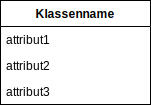
\includegraphics{Bilder/Kapitel-4/darstellung_klasse_mit_drei_attributen.pdf}
	\caption[Die UML-Darstellung einer Klasse]{Die UML-Darstellung einer Klasse mit Angabe des Namens der \mbox{Klasse} und drei Attributen}
	\label{fig:darstellung_klasse_mit_drei_attributen}
\end{figure}

In der UML-Darstellung wird das Rechteck der Klasse durch eine Linie horizontal unterteilt. Oberhalb der Linie steht der schon bekannte Name der Klasse, unterhalb der Linie werden die Attribute, untereinander und linksbündig gesetzt, aufgeführt. Jedes (spätere) Objekt, das nach den Vorgaben der Klasse modelliert wird – man sagt verkürzend: „Jedes Objekt der Klasse“ – verfügt über genau die Attribute, die die Klasse definiert. Die Werte der Attribute, also die Ausprägung der Merkmale, sind dabei jedoch spezifisch pro Objekt.

Wir wechseln von Katzen zu Autos! Abbildung~\ref{fig:klasse_auto_mit_zwei_attributen} zeigt eine Klasse \sttpUMLText{Auto} mit den zwei Attributen \sttpUMLText{modell} und \sttpUMLText{farbe}.

\begin{figure}[h!]
	\centering
	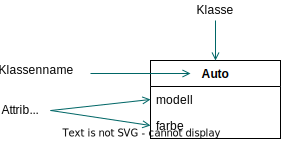
\includegraphics{Bilder/Kapitel-4/klasse_auto_mit_zwei_attributen.pdf}
	\caption{Eine Klasse \sttpUMLText{Auto} mit zwei Attributen}
	\label{fig:klasse_auto_mit_zwei_attributen}
\end{figure}

Abbildung~\ref{fig:drei_mal_klasse_auto_plus_klasse_hugoauto} oben zeigt mit \sttpUMLText{ellensAuto}, \sttpUMLText{heikesAuto} und \sttpUMLText{marvinsAuto} drei Objekte, die die von der Klasse \sttpUMLText{Auto} definierten Merkmale (Vorhandensein der Eigenschaften Modell und Farbe) erfüllen und damit Objekte der Klasse \sttpUMLText{Auto} sind. Die von der Klasse vorgegebenen Attribute sind bei den Objekten mit konkreten Werten belegt: Für das Attribut \sttpUMLText{modell} finden wir hier die Werte Toyota Yaris und VW Golf, für das Attribut \sttpUMLText{farbe} die Werte stahlblau, weiß und rot. Wie hier bei dem \sttpUMLText{modell}-Attribut von \sttpUMLText{ellensAuto} und \sttpUMLText{heikesAuto} können die Werte -- man sagt auch synonym: Wertebelegungen
\marginline{Werte\-belegungen}
-- von Attributen bei unterschiedlichen Objekten auch übereinstimmen. Wenn zwei Objekte derselben Klasse in \textbf{allen} \mbox{Wertebelegungen} der Attribute übereinstimmen, also zum Beispiel Heikes Toyota Yaris auch stahlblau wäre wie der von Ellen, nennt man dies in der Objektorientierung zustandsgleiche Objekte.

\begin{figure}[h!]
	\centering
	\includegraphics{Bilder/Kapitel-4/klasse_auto.pdf}
	\caption[Drei Objekte der Klasse \sttpUMLText{Auto}]{Drei Objekte der Klasse \sttpUMLText{Auto} (oben) und ein Objekt mit Namen \sttpUMLText{hugosAuto}, das kein Objekt der Klasse Auto aus Abbildung~\ref{fig:klasse_auto_mit_zwei_attributen} ist (unten)}
	\label{fig:drei_mal_klasse_auto_plus_klasse_hugoauto}
\end{figure}

Abbildung~\ref{fig:drei_mal_klasse_auto_plus_klasse_hugoauto} unten
\marginline{der Unterschied zwischen Realwelt-Objekten und modellierten Objekten}
zeigt ein Objekt mit Namen \sttpUMLText{hugosAuto}, das im Gegensatz zu den drei anderen Objekten kein Objekt der in Abbildung~\ref{fig:klasse_auto_mit_zwei_attributen} modellierten Klasse \sttpUMLText{Auto} ist, da es über ein Attribut \sttpUMLText{baujahr} verfügt, das die in Abbildung~\ref{fig:klasse_auto_mit_zwei_attributen} dargestellte Auto-Klasse nicht kennt. An dieser Stelle müssen Sie sich noch einmal den Unterschied zwischen Realwelt-Objekten und den für Softwareengineering-Zwecke modellierten Objekten vergegenwärtigen: Das Realwelt-Auto von Hugo ist sicher genau wie die Autos von Ellen, Heike und Marvin ein Auto. Und die Realwelt-Autos der drei letzteren Personen haben auch genau wie Hugos Auto ein Baujahr. Die in Abbildung~\ref{fig:klasse_auto_mit_zwei_attributen} für einen (hier unbekannten) Zweck im Rahmen des Softwareengineering modellierte Klasse Auto abstrahiert von allen Eigenschaften von Realwelt-Autos, die für den Modellierungszweck nicht relevant sind. Und in diesem Beispiel betrifft das eben auch das Merkmal Baujahr. \textbf{Modellierte} Objekte vom Typ Auto besitzen hier daher kein Attribut \sttpUMLText{baujahr}, auch wenn für ihre Realweltentsprechungen ein Baujahr existiert.

An dem Auto-Baujahr-Beispiel zeigt sich ein weiterer praktischer Verwendungszweck von Objektdiagrammen. In  Diskussionen über die relevanten Strukturen der Domäne zwischen Softwareentwicklungsteam und Kunden kann es für die Kunden schwierig sein, die ihnen bekannte Ebene der Realwelt-Objekte mit der Ebene der deutlich abstrakteren Klassen zusammenzubringen. Hier kann es helfen, statt Klassen zunächst konkrete (Beispiel)Objekte und ihre Eigenschaften zu modellieren und erst anschließend auf dieser Grundlage die benötigten Klassen zu entwerfen.
